\subsubsection{The slab detachment benchmark}
\label{sec:benchmark_slab_detachment}

\textit{This section was contributed by Cedric Thieulot and Anne Glerum.}

Slab detachment (slab break-off) may occur in the final stages of subduction
as a consequence of the combination of a buoyant crust and strong slab pull.
It is often invoked to explain
geophysical and geological observations such as
tomographic images of slab remnants and
exhumed ultra-high-pressure rocks \cite{wosp00,vaal11,garm18}.

This benchmark is based on the setup by S. Schmalholtz \cite{schm11}, which was subsequently
run with \aspect{} by A. Glerum \cite{gltf18}.
The computational domain is a $1000 \si{km}\times 660 \si{km}$ box.
No-slip boundary conditions are imposed on the sides of the system, while free-slip
boundary conditions are imposed at the top and bottom.

\begin{figure}
\centering
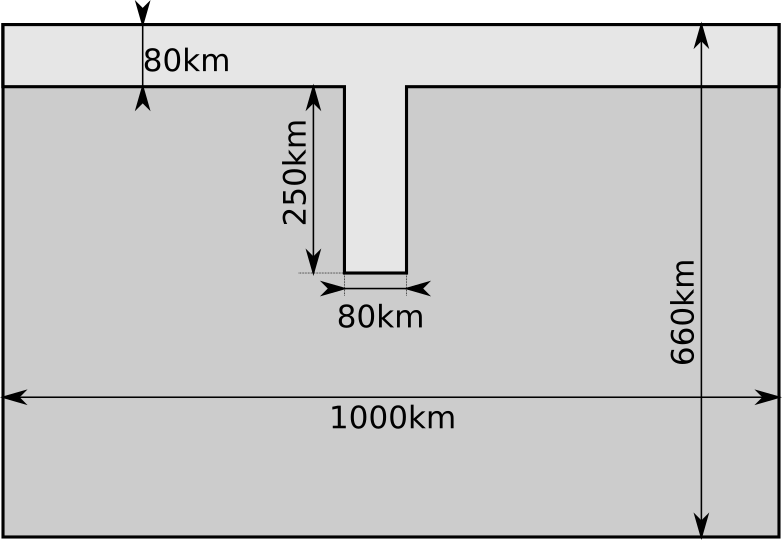
\includegraphics[width=0.6\linewidth]{cookbooks/benchmarks/slab_detachment/doc/drawing.png}
\caption{\it Slab detachment benchmark: Initial geometry
\label{fig:slab_detachment_setup}}
\end{figure}

Two materials are present in the domain: the lithosphere and the mantle as shown
in Figure~\ref{fig:slab_detachment_setup}. The gravity acceleration
is Earth-like with $g=9.81 \si{m}\si{s}^2$.
The overriding plate is $80\si{km}$ thick and is placed at the top of the domain.
The already subducted lithosphere extends vertically into the mantle for $250 \si{km}$.
This slab has a density $\rho_s=3300\si{kg}/\si{m}^3$ and is characterized by a power-law flow law so that
its effective viscosity depends on the square root of the second invariant
of the strainrate $\dot\varepsilon$:
\[
\eta_{eff} = \eta_0 \, \dot\varepsilon^{1/n-1}
\]
with $n=4$ and $\eta_0=\SI{4.75e11}{Pa . s}$.
The mantle occupies the rest of the domain and has a constant viscosity $\eta_m=\SI{1e21}{Pa . s}$
and a density $\rho_m=\SI{3150}{kg/m^3}$. Viscosity is capped between $\SI{1e21}{Pa . s}$ and $\SI{1e25}{Pa . s}$.
Figure~\ref{fig:slab_detachment_evolution} shows the various fields and their evolution through time.
As shown in \cite{schm11,gltf18} the hanging slab necks, helped by the localizing effect of the
nonlinear rheology. Model results were shown to compare favorably to the results of \cite{schm11} in \cite{gltf18,hitg14}
and the effect of viscosity and material averaging was explored in \cite{gltf18}.

\begin{figure}
\caption{\it Slab detachment benchmark: a,b) velocity and strain rate fields at $t=0$.
c,d,e) and f,g,h) time evolution of the viscosity and slab composition fields at $t=0, 6, 12\text{Myr}$.
\label{fig:slab_detachment_evolution}}
\end{figure}


